%!TEX root = ../dissertation.tex

\chapter{Background}
\label{chp:background}

This chapter introduces and describes the foundational knowledge necessary to fully understand the topics presented in this thesis. It begins by defining the notations used throughout the subsequent chapters. Following this, it provides an overview of machine learning and supervised classification, including a detailed explanation of the \acs{$k$-NN} classifier. Finally, it addresses the safety and fairness issues associated with these methods, and outlines the properties that must be evaluated as a result.


\section{Notation}
\label{sec:notation}

An $n$-dimensional vector space $\mathcal{X} \subseteq \mathbb{R}^n$, called \textit{input feature space}, and a set of classification labels $\mathcal{L} \subset \mathbb{N}$ are assumed. Vectors in this input feature space are denoted with bold letters while natural numbers are denoted with normal letters. Given vectors $\vec{x}, \vec{y} \in \R[n]$, and a constant $c \in \R$:

\begin{itemize}
  \item $\forall i \in \{1, n\}\ \ \vec{x}_i \in \mathbb{R}$ denotes the $i$-th component of $\vec{x}$;
  \item $\vec{x} \cdot \vec{y} \doteq \sum_{i=1}^n \vec{x}_i + \vec{y}_i$ represents the dot product between two vectors;
  \item $\vec{x} + \vec{y} \doteq (\vec{x}_1 + \vec{y}_1, \vec{x}_2 + \vec{y}_2, \ldots,\vec{x}_n + \vec{y}_n)$ is the vector addition of two vectors;
  \item $\vec{x} + c \doteq (\vec{x}_1 + c, \vec{x}_2 + c, \ldots,\vec{x}_n + c)$ denotes the summation between a vector and constant;
  \item $c\cdot \vec{x} \doteq (c\cdot\vec{x}_1, c\cdot\vec{x}_2, \ldots,c\cdot\vec{x}_n)$ denote the multiplication between a constant;
  \item $\lVert \vec{x} \rVert_2 = \sqrt{\vec{x} \cdot \vec{x}}$ denotes the $\ell_2$ (i.e., Euclidean) norm;
  \item $\lVert \vec{x} \rVert_\infty = \max\{|\vec{x}_i| ~|~ i \in \{1, n\}\}$ is $\ell_\infty$ (i.e., maximum) norm;
\end{itemize}

\noindent A dataset will be denoted as $\mathcal{S} = \{\vec{z}^{(i)}\}_{i=1}^n = \{(\vec{x}^{(i)}, l^{(i)}) \}_{i=1}^n \subset \mathcal{Z} = \mathcal{X} \times \mathcal{L}$. Given a dataset $\mathcal{S}$:
\begin{itemize}
	\item $\mathcal{S}_X$ denotes the samples in the dataset $\mathcal{S}$;
	\item $\mathcal{S}_L$ denotes the labels in the dataset $\mathcal{S}$;
\end{itemize}
\noindent If not specified otherwise, $\mathcal{S}, \mathcal{T}$ will denote the training set and the test set respectively.

\noindent Given $\vec{n} \in \R, b \in \N$ let
\[
	\pi_{\vec{n},b} = \vec{n}_1x_1 + \vec{n}_2x_2 + \cdots + \vec{n}_nx_n + b = 0
\]
be the equation of a hyperplane. Then $\pi_{\vec{n},b}(\vec{y}) = n_1\cdot y_1 + n_2\cdot y_2 + \cdots + n_n \cdot y_n + b$

\section{Machine Learning}
\label{sec:ml}

\begin{figure}[H]
	\centering
	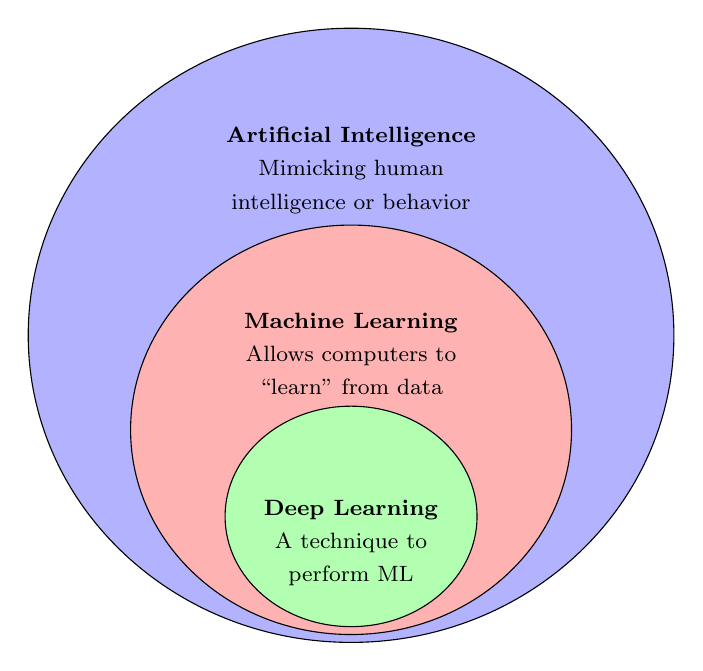
\begin{tikzpicture}
		\def\firstellipse{(1,-1.1) ellipse (1.6 and 1.4)}
		\def\secondellipse{(1,0) ellipse (2.8 and 2.6)}
		\def\thirdellipse{(1,1.2) ellipse (4.1 and 3.9)}
		\filldraw[fill=blue!30]\thirdellipse;
		\filldraw[fill=red!30]\secondellipse;
		\filldraw[fill=green!30]\firstellipse;
		\node at (1,-2.23) [label={[align=center] \footnotesize \textbf{Deep Learning} \\ \footnotesize A technique to \\ \footnotesize perform ML}]{};
		\node at (1,0.2) [label={[align=center] \footnotesize \textbf{Machine Learning} \\ \footnotesize Allows computers to \\ \footnotesize ``learn'' from data}]{};
		\node at (1,2.5) [label={[align=center] \footnotesize \textbf{Artificial Intelligence} \\ \footnotesize Mimicking human \\ \footnotesize  intelligence or behavior}]{};
	\end{tikzpicture}
	\caption[Venn diagram showing the relation between artificial intelligence, machine learning and deep learning]{Venn diagram showing the relation between artificial intelligence, machine learning and deep learning.}
	\label{fig:ai-ml-dl}
\end{figure}

In contemporary discourse, artificial intelligence (\acs{AI}), machine learning, and deep learning are increasingly prevalent terms. While often confused or used interchangeably, these concepts are, in fact, distinct.

Artificial intelligence is a rapidly expanding field with numerous practical applications and active research areas. As defined by its pioneer, John McCarthy \cite{mccarthy2004artificial}:
\begin{center}
	\itshape
	``The science and engineering of making intelligent machines, especially intelligent computer programs.''
\end{center}
Its main goal is to employ diverse technologies to develop machines and computers capable of replicating cognitive functions associated with human intelligence, thereby automating mind- and time-consuming tasks. \acs{AI} is particularly suited for solving problems that are intellectually challenging for humans but readily definable in a formal mathematical manner understandable by computers. Conversely, tasks that our minds perform effortlessly, such as recognizing objects, faces, or sounds, categorizing document subjects, or identifying entities (places, titles, names, actions, etc.) in phrases or images, pose a challenge in formalization for computer understanding. This is because we learn these tasks through development and experience. The real challenge arises when precise problem formalization is impossible, when input or output uncertainty exists, and when solutions are excessively complex or inefficient.

Machine learning is a subset of artificial intelligence designed to address these challenges. \acs{ML} focuses on creating systems or models that learn inherent data patterns and improve performance in specific tasks without explicit programming. These models learn from past experiences or examples to make decisions on new data, contrasting with traditional AI methods where human programmers write rules to transform input data into desired results. The underlying assumption is that a stochastic process governs real-world data, and machine learning methods approximate this process by learning patterns and correlations within available data (a representation of real-world data). The learned process is then used to make predictions on unseen samples. Data is therefore crucial in \acs{ML} model learning, commonly represented as sets of $n$-dimensional vectors in $\mathbb{R}^n$ where each vector component is called \emph{attribute} or \emph{feature}. For example, the features of an image, represented as a vector, can be its pixels ranging from $0$ to $255$.

\noindent Data and tasks determine which \acs{ML} method is most suitable and performing for each specific case. Within machine learning, the following learning paradigms are identified:
\begin{itemize}
	\item \textbf{Supervised learning:} data is presented as a set of examples $\bigcup_{i=1}^n\{(\vec{x}^{(i)}, l^{(i)})\}$ known as the training set. Each example is a pair consisting of an input feature vector from $\mathcal{X}$ and its corresponding output, typically a label. Supervised learning is particularly well-suited for classification and regression tasks: a classification function is learned for discrete outputs, while a regression function is learned for continuous outputs. The learned function is then used to predict the output for unseen data.;
	\item \textbf{Unsupervised learning:} data are presented as a set of unlabelled vectors $\bigcup_{i=1}^n\{\vec{x}_i\}$. In this scenario, the outputs represent the inherent data structure, determined by minimizing a cost function. Unsupervised learning is particularly well-suited for clustering and dimensionality reduction tasks;
	\item \textbf{Reinforcement learning:} as for unsupervised learning, data are presented as a set of unlabelled vectors $\bigcup_{i=1}^n\{\vec{x}_i\}$. In contrast, however,A scalar reward signal is used to evaluate these pairs through trial and error, aiming to find the optimal prediction for each input. This approach is employed in domains where systems must adapt to environmental changes, and is thus applicable to problems ranging from control systems to game playing.
\end{itemize}

There several machine learning methods, and deep learning is one of them, but we will focus on its use for supervised classification tasks, precisely exploiting the $k$ nearest neighbors algorithm. For more in depth introduction to machine learning refer to \cite{alpaydin2020introduction}.

\subsection{Supervised Classification}
\label{subsec:supervised-class}

Classification is the process of assigning a category to a new sample based on its likelihood of belonging to that category. The goal is to learn a mapping from inputs $\vec{x} \in \mathcal{X}$ to a label $l_{\vec{x}}$ representing a category, using a labeled training dataset $T=\bigcup_{i=1}^n\{(\vec{x}^{(i)}, l^{(i)})\}$. This task can be formalized as approximating an unknown function $f\colon \mathcal{X} \rightarrow \wp(\mathcal{L})$, which perfectly predicts the label for a given input (i.e.,$f(\vec{x}^{(i)}) = l^{(i)}\ \ \forall\ (\vec{x}^{(i)}, l^{(i)}) \in T$). This is achieved by selecting a function $h \colon \mathcal{X} \rightarrow \wp(\mathcal{L})$ from the hypothesis space, which encompasses all possible functions, such that $h$ approximates $f$ as closely as possible on the training data. The number of possible outputs determines the type of supervised classification: \emph{binary classification} occurs when each data instance can be assigned to one of two possible class labels; \emph{multiclass classification} involves more than two class labels, with each instance assigned to only one. \emph{Multilabel classification} addresses cases where a single example can belong to multiple classes. However, this thesis focuses solely on binary and multiclass classification.


\subsection{K-NN Classifiers}
\label{subsec:knn-classifiers}

One of the simplest and most trivial forms of learning for classification tasks is rote learning \cite{daniels2015rote}, which involves memorizing the entire training data and performing classification only if the attributes of the test sample exactly match those of a training example. This approach has two significant drawbacks: many test samples will remain unclassified due to the lack of an exact match with any training example, and when two or more training examples have identical attributes but different class labels, it becomes impossible to infer the correct label. A possible solution to mitigate these issues is to employ a more refined approach based on similarity rather than strict equality.

The $k$-nearest neighbors algorithm is a \emph{non-parametric} supervised learning method that leverages data similarity to make classifications or predictions about the grouping of an individual sample, operating under the assumption that similar data should be classified similarly. The term 'non-parametric' indicates that no assumptions are made about the underlying data distribution from which the dataset is sampled. Consequently, the model structure is uniquely determined by the dataset itself, which is highly advantageous in practice, as most real-world datasets do not conform to predefined mathematical models. A \acs{$k$-NN} classifier assigns an unknown feature vector $\vec{x} \in \mathbb{R}^n$ into the class $y_{\vec{x}}$​ to which the majority of its $k$ nearest neighbors belong, thus preventing the algorithm from failing when there is no exact match. In its simplest form, the $1$-NN classifier, it assigns a test sample the class of its closest neighbor. The number $k \in \mathbb{N}$  of neighbors, as well as the similarity metric used to compare vectors in $\mathbb{R}^n$, are hyperparameters of this prediction model. The most commonly used similarity metrics are


\begin{itemize}
  \item \textbf{Euclidean distance} (i.e. $\ell_2$ norm): This metric computes the straight-line distance between two points of a vector space, and suitable for data that has continuous and numerical attributes with similar scales and ranges;
  \item \textbf{Manhattan distance} (i.e. $\ell_1$ norm): This metric computes the distance between two points of a vector space in a grid-like path, and is preferred for data that has discrete and categorical attributes;
  \item \textbf{Cosine similarity}: This metric calculates the cosine of the angle between two vectors of a vector space, and it excels in sparse, high-dimensional data like text or images, focusing on direction rather than magnitude.
\end{itemize}

As Sebastian Raschka pointed out \cite{raschka2018stat}, although technically \emph{plurality voting} is used, the term \emph{majority voting} is almost ubiquitous in literature. The difference between these two terms is that ``majority voting'' requires a majority of more than $50\%$, which only works when there are only two classes. When there are multiple classes, e.g. four categories, it is not always necessary a $50\%$ of the vote to make a decision about a class, and it is in fact possible to assign a class label with a vote of more than $25\%$.

The left picture in \autoref{fig:knn-example} illustrates a classification performed using a k-NN model with $k=3$ and Euclidean distance as the similarity metric, applied to a dataset in $\mathbb{R}^2$ with three classes: \emph{red}, \emph{green}, and \emph{blue}. By applying the $3$-NN algorithm to every vector in the input space, the right picture depicts the dataset after classification. For an unknown input vector, represented by a gray dot in the left picture, the algorithm computes the 3 nearest samples in the dataset, which are those within the dashed circle, and then infers the most common label among them. Following this strategy, it's possible that two or more labels receive an equal number of votes, resulting in a tie. For example, replacing a red point inside the dashed circle with a blue point would create a tie, as each label would receive exactly $1$ vote.

\begin{figure}[H]
	\centering
	\usetikzlibrary{arrows.meta, intersections}
	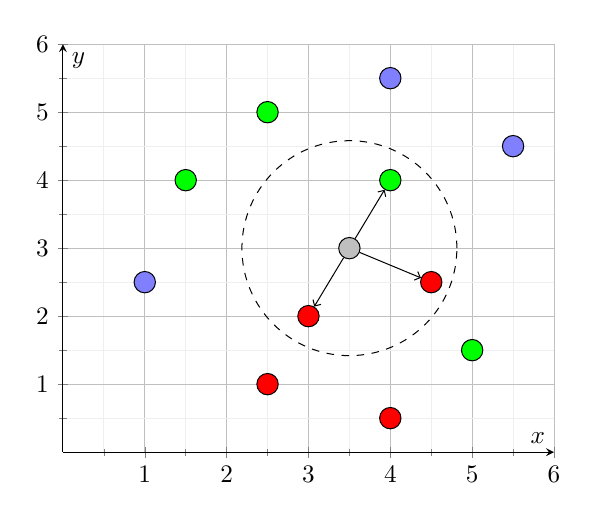
\begin{tikzpicture}[
		scale = 0.91,
		> = {Straight Barb[scale=0.8]},
		dot/.style = {circle, draw, fill=#1, inner sep=3pt, node contents={}}
	]
		\begin{axis}[
			xmin = 0, xmax = 6,
			ymin = 0, ymax = 6,
			xtick distance = 1,
			ytick distance = 1,
			grid = both,
			minor tick num = 1,
			major grid style = {lightgray},
			minor grid style = {lightgray!25},
			axis x line=center,
			axis y line=center,
			xlabel = {$x$},
			ylabel = {$y$},
			xlabel style={above left},
			ylabel style={below right}
		]
			\node (m) at (3.5,3) [dot=gray!50];
			\node (c) at (3.5,3) [circle, draw, dashed, inner sep=0pt, minimum size=3cm, name path=C] {};
			\node (p1) at (2.5,5) [dot=green];
			\node (p2) at (4,4) [dot=green];
			\node (p3) at (5,1.5) [dot=green];
			\node (p4) at (1.5,4) [dot=green];
			\node (p5) at (1,2.5) [dot=blue!50];
			\node (p6) at (4,5.5) [dot=blue!50];
			\node (p6) at (5.5,4.5) [dot=blue!50];
			\node (p7) at (4,0.5) [dot=red];
			\node (p8) at (4.5,2.5) [dot=red];
			\node (p9) at (3,2) [dot=red];
			\node (p10) at (2.5,1) [dot=red];
			\draw [->] (m) -- (p2);
			\draw [->] (m) -- (p8);
			\draw [->] (m) -- (p9);
		\end{axis}
	\end{tikzpicture}
    \qquad
    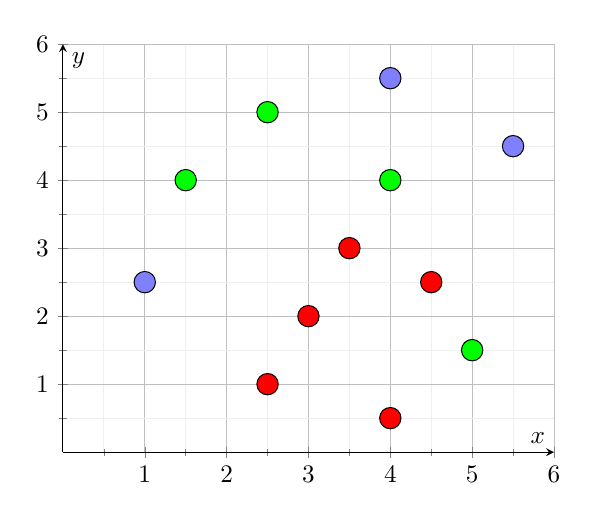
\begin{tikzpicture}[
   		scale = 0.91,
   		> = {Straight Barb[scale=0.8]},
   		dot/.style = {circle, draw, fill=#1, inner sep=3pt, node contents={}}
   	]
    	\begin{axis}[
    		xmin = 0, xmax = 6,
    		ymin = 0, ymax = 6,
    		xtick distance = 1,
    		ytick distance = 1,
    		grid = both,
    		minor tick num = 1,
    		major grid style = {lightgray},
    		minor grid style = {lightgray!25},
    		axis x line=center,
    		axis y line=center,
    		xlabel = {$x$},
    		ylabel = {$y$},
    		xlabel style={above left},
    		ylabel style={below right}
    		]
    		\node (m) at (3.5,3) [dot=red];
    		\node (p1) at (2.5,5) [dot=green];
    		\node (p2) at (4,4) [dot=green];
    		\node (p3) at (5,1.5) [dot=green];
    		\node (p4) at (1.5,4) [dot=green];
    		\node (p5) at (1,2.5) [dot=blue!50];
    		\node (p6) at (4,5.5) [dot=blue!50];
    		\node (p6) at (5.5,4.5) [dot=blue!50];
    		\node (p7) at (4,0.5) [dot=red];
    		\node (p8) at (4.5,2.5) [dot=red];
    		\node (p9) at (3,2) [dot=red];
    		\node (p10) at (2.5,1) [dot=red];
    	\end{axis}
    \end{tikzpicture}
	\caption[3NN over a dataset with 3 classes, which shows how a new  point is classified (left), as well as its label after being classified (right)]{3NN over a dataset with 3 classes, which shows how a new  point is classified (left), as well as its label after being classified (right).}
	\label{fig:knn-example}
\end{figure}

As can be seen from the example above, a \acs{$k$-NN} model does not need a learning phase, which is instead required in most supervised \acs{ML} algorithms, because all the examples are stored and entirely used at classification time, a feature that makes $k$-NN a so-called \emph{lazy} (or \emph{just-in-time}) learning algorithm \cite{bontempi}. While this makes it quite simple to implement, it can potentially result in a high computation time due to the effort of computing and sorting the distances, especially when so many neighbors must be found. For this reason, $k$ is usually a low value, very often below $9$ and in any case always smaller than the square root of the total number of samples in the dataset. Being lazy, on the other hand, makes it perform well in many situations. Under certain reasonable assumptions, a well-known result by Cover and Hart \cite{cover1967} shows that the classification error of the nearest neighbor rule is bounded above by twice the optimal Bayes error. Furthermore, the error of the general \acs{$k$-NN} method approaches that of the Bayes error asymptotically and can be used to approximate it.
\vspace{6pt}

\autoref{alg:knn} provides a high-level summary of the \acs{$k$-NN} algorithm for classification tasks. Given a ground truth dataset $T = \{(\vec{x}_1, l_1),\dots, (\vec{x}_{N}, l_N)\} \subseteq X \times L$, a number of neighbors $k\in \mathbb{N} \smallsetminus \{0\}$, and a distance function $\delta\colon X \times X \rightarrow \mathbb{R}_{\geq 0}$, a $k$-NN classifier is modeled as a total function $C_{T, k, \delta}\colon X \rightarrow \wp(L)$, which maps an input sample $\vec{x} \in X$ into a nonempty set of labels, by first selecting the similarly $k$ samples in $D$ to the input $\vec{x}$ according to $\delta$ metric, and then computing the set of their most frequent labels.  Since a tie vote means to output a set including more than one label, we consider sets of labels as co-domain of classifiers.

\begin{algorithm}[H]
	\caption[$k$-NN algorithm]{\acs{$k$-NN} algorithm}
	\label{alg:knn}
	\begin{algorithmic}[1]
    \Require{$D$: the dataset, $\delta$: the similarity metric, $\vec{x}$: The input sample}
    \Ensure{The possible classifications of the input samples}

    \State $M, O \gets \varnothing$
		\ForAll {$(\vec{y}, l_{\vec{y}}) \in D$}
			\State $d \gets \delta(\vec{x}, \vec{y})$
			\State $O \gets O \cup (d, l{\vec{y}})$
		\EndFor
		\State $O.\textsc{Sort}()$
		\ForAll {$i \in \{1,\ldots,k\}$}
			\State $M[i] \gets O.\textsc{Extract}[i]$
		\EndFor
		\State \Return $\argmax\limits_{l \in L} \sum_{(\vec{y}, l_{\vec{y}}) \in M \textbf{ s.t. } l = l_{\vec{y}}} 1$
	\end{algorithmic}
\end{algorithm}


\subsection{Adversarial Examples}
\label{subsec:adv-examples}

Adversarial examples in machine learning are inputs to a model that are intentionally designed to cause the algorithm make mistakes in its predictions, yet appearing to be a legitimate input to a human. In this thesis, we will look at these kinds of inputs in the context of \acs{$k$-NN} classifiers. Given a classifier $C\colon X \rightarrow \wp(L)$, adversarial examples can be formally defined as inputs $\bar{\vec{x}}$ where the difference between $\bar{\vec{x}}$ and non-adversarial inputs $\vec{x}$ is minimal under some distance metric $\delta\colon X \times X \rightarrow \mathbb{R}_{\geq 0}$, but enough to make $C$ infer a different output. To obtain such an $\bar{\vec{x}}$, a \emph{perturbation} $P$ is applied to $\vec{x}$ to cause a variation in the feature values of $\vec{x}$, defining a potential adversarial region $P(\vec{x}) \subseteq X$ in which $\bar{\vec{x}}$ belong. Generally, adversarial examples attempt to satisfy:
\begin{equation*}
	0 < \delta(\vec{x}, \bar{\vec{x}}) \leq \epsilon \text{ such that } C(\vec{x}) \neq C(\bar{\vec{x}})
\end{equation*}
where $\epsilon \in \mathbb{R}$ is a (small) constant bounding the magnitude of the perturbation.

Resilience to adversarial perturbations is a key property of a robust machine learning model. Ideally, the classifier should maintain consistent decisions despite minor variations in the input features. While this property is often assumed, it is not always guaranteed. For example, when the distance function is overly simplistic, \acs{$k$-NN} can be significantly affected by adversarial perturbations, especially when dealing with feature vectors that have limited precision. In digital images, for instance, each pixel is typically represented with only $8$ bits, with values from $0$ to $255$, discarding all information below $1/255$ of the dynamic range. As a result, if we consider a perturbation $\tau > 0$ smaller than this threshold, it would be unrealistic for the classifier to differentiate between an input vector $\vec{x}$ and a perturbed vector $\bar{\vec{x}} = \vec{x} + \vec{y}$, as long as every element of $\vec{y}$ is smaller than or equal to $\tau$. However, if the distance between vectors is computed by, for example, summing their feature-wise differences, as happens using the Manhattan distance, then $\delta(\vec{x}, \vec{x} + \vec{y})$  is the same whether we add $n\tau$ to the first feature or distribute $\tau$ across all features of $\vec{x}$. This behavior is problematic because, despite the differences in how perturbations affect the features, the distance metric treats them as equally significant, leading to potentially misleading results.

In this study, we model the adversarial region using the well-known $\ell_\infty$-perturbation \cite{carlini}, which uniformly affects all features. Given an input vector $\vec{x} \in \mathbb{R}^n$ and a perturbation magnitude $\epsilon \geq 0$, the $\ell_\infty$-perturbation defines the adversarial region as $P^\epsilon_\infty(\vec{x}) \triangleq \{\vec{w} \in \mathbb{R}^n \mid \max(|\vec{w}_1 - \vec{x}_1|, \dots, |\vec{w}_n - \vec{x}_n|) \leq \epsilon \}$, which represents the $\ell_\infty$-ball of radius $\epsilon$ centered at $\vec{x}$. This approach accounts for all possible combinations of perturbed features, where each feature of the input sample can be perturbed up to the magnitude $\epsilon$.


\subsection{Stability and Robustness}
\label{subsec:stab-rob}

Classifiers are usually evaluated and compared through multiple metrics. A simple and intuitive metric is \emph{accuracy} on a test set: given ground truth test dataset $T = \{(\vec{x}_1, l_1),\dots, (\vec{x}_{n}, l_n)\} \subseteq \mathcal{X} \times \mathcal{L}$, the accuracy of a classifier $C\colon X \rightarrow \wp(L)$ on $T$  is defined by the ratio:
\begin{equation}\label{eq:accuracy}
	\textsc{Accuracy}(C, T) \triangleq \frac{|\{(\vec{x},l_{\vec{x}}) \in T ~|~ C(\vec{x}) = \{l_{\vec{x}}\}|}{|T|}
\end{equation}
that is the proportion of samples with correct predictions to the total number of samples. In adversarial scenarios, assessing a classification model solely on this standard metric is far from adequate. Although accuracy is useful in assessing the model's overall performance, it does not highlight any safety concerns. We now define two relevant properties in this context, which will be formally certified by our method.

\begin{definition}[Stability]
	\label{def:stability}
	A classifier $C\colon X \rightarrow \wp(L)$ is \emph{stable} on an input $\vec{x} \in X$ for a given perturbation $P\colon X \rightarrow \wp(X)$, denoted by $\textsc{Stable}(C, P, \vec{x})$, when $\forall \bar{\vec{x}} \in P(\vec{x}).\: ~ C(\bar{\vec{x}}) = \{l\}$ holds for some $l \in L$.
\end{definition}

\begin{definition}[Robustness]
	\label{def:robustness}
	A classifier $C\colon X \rightarrow \wp(L)$ is \emph{robust} on an input $(\vec{x}, l_{\vec{x}}) \in X \times L$ for a given perturbation $P\colon X \rightarrow \wp(X)$, denoted by $\textsc{Robust}(C, P, \vec{x}, l_{\vec{x}})$, when $\forall \bar{\vec{x}} \in P(\vec{x}).\: ~ C(\bar{\vec{x}}) = \{l_{\vec{x}}\}$ holds.
\end{definition}

Stability means that a classifier does not change its output on a region of similar inputs, and it is orthogonal to accuracy in the sense that it does not require prior knowledge of the ground truth labels. Robustness, on the other hand, requires the classifier to be stable and correct, which means that it must output the same label that the input has in the dataset to which it belongs. It should be noted that for null $\ell_\infty$-perturbations, i.e. with $\epsilon = 0$, the definitions of accuracy and robustness coincide, leading us to conclude that the latter property expresses accuracy in adversarial scenarios.

As we did in \eqref{eq:accuracy}, we define the stability and robustness of $C$ on some test set $T \subseteq X \times L$ by the ratios:
\begin{equation}\label{eq:stab-rob}
	\begin{aligned}
		\textsc{Stability}(C, T) &\triangleq \frac{|\{(\vec{x},l_{\vec{x}}) \in T ~|~ \textsc{Stable}(C, P, \vec{x})\}|}{|T|} \\
		\textsc{Robustness}(C, T) &\triangleq \frac{|\{(\vec{x},l_{\vec{x}}) \in T ~|~ \textsc{Robust}(C, P, \vec{x}, l_{\vec{x}})\}}{|T|}
	\end{aligned}
\end{equation}
It is worth remarking that if we have a tie vote using the \acs{$k$-NN} algorithm, $|C(\vec{x})| > 1$ always holds, and hence $C$ can be neither stable nor robust on $\vec{x}$ by definition.


\subsection{Individual Fairness}
\label{subsec:fairness}

When it comes to \emph{individual fairness} of \acs{ML} classifiers, as the name suggests, we want to know if similar inputs will receive a similar class label. The similarity relation on the input space $X$ is expressed in terms of a distance $\delta$ and a threshold $\epsilon>0$  by considering $S_{\delta, \epsilon} \triangleq \{(\vec{x}, \vec{y}) \in X \times X ~|~ \delta(\vec{x}, \vec{y}) \leq \epsilon\}$.  According to Dwork's work \cite{dwork2012fairness}, a model is \emph{biased} (or \emph{unfair}) if there is a pair of valid inputs that are close to each other for some distance function $\delta$, but are treated differently by the model, leading to a different outcome, and it is instead \emph{unbiased} (or \emph{fair}) if such a pair does not exist. Consequently, given an input $\vec{x} \in X$, we say that a classifier $C: X \rightarrow \wp(L)$ is fair on $\vec{x}$ with respect to $S_{\delta, \epsilon}$ when:
\begin{equation*}
	\forall \vec{y} \in X.\: (\vec{x}, \vec{y}) \in S_{\delta, \epsilon} \Rightarrow C(\vec{x}) = C(\vec{y}).
\end{equation*}

Following the above consideration, we now formally define the individual fairness property in adversarial scenarios.

\begin{definition}[Individual Fairness]
	\label{def:fairness}
	Given an input $\vec{x} \in X$ and perturbation $P\colon X \rightarrow \wp(X)$ such that $P_{\delta, \epsilon}(\vec{x}) \triangleq \{\vec{y} \in X ~|~ \delta(\vec{x}, \vec{y})\}$ for some distance function $\delta$, a classifier $C: X \rightarrow \wp(L)$ is \emph{fair} on $(\vec{x}, l_{\vec{x}})$ with respect to $P_{\delta, \epsilon}$, denoted by $\textsc{Fair}(C, P_{\delta, \epsilon}, \vec{x})$, when $\forall \bar{\vec{x}} \in P_{\delta, \epsilon}(\vec{x}).\: ~ C(\vec{x}) = C(\bar{\vec{x}})$ holds.
\end{definition}

By leveraging on Definition \ref{def:fairness}, we observe that individual fairness boils down to stability, namely, for all inputs $\vec{x}$, $\textsc{Fair}(C, P_{\delta, \epsilon}, \vec{x}) \Leftrightarrow \textsc{Stable}(C, P_{\delta, \epsilon}, \vec{x})$ holds. For the individual fairness metric on a given test set $T \subseteq X \times L$ we therefore have that:
\begin{equation}\label{eq:fairness}
	\textsc{fairness}(C, T) \triangleq \frac{|\{(\vec{x}, l_{\vec{x}}) \in T ~|~ \textsc{Fair}(C, P_{\delta, \epsilon}, \vec{x})\}|}{|T|}
\end{equation}

In our experiments, we have considered the \textsc{Noise-Cat} similarity relation as defined in~\cite{ruoss2020learning}, where two inputs $\vec{x}, \vec{y} \in X$ are similar when: \textbf{(i)} given a subset $N \subseteq \mathbb{N}$ of indexes of numerical features and a threshold $\epsilon \in \mathbb{R}_{\geq 0}$, for all $i \in N$, $|\vec{x}_i - \vec{y}_i| \leq \epsilon$;
\textbf{(ii)}~given a subset $C \subseteq \mathbb{N}$ of indexes of categorical features, both $\vec{x}$ and $\vec{y}$ are allowed to have any category for features with indexes in $C$;
\textbf{(iii)}~every other feature of $\vec{x}$ and $\vec{y}$,
i.e. with index not in $N$ nor $C$, must be the same, namely, for any index
$i \not\in (N \cup C)$, $\vec{x}_i = \vec{y}_i$ holds.
For example, if we wanted to make a classification for statistical purposes, two individuals having two numerical features \emph{age} and \emph{height} and two categorical features \emph{gender} and \emph{country}, could be considered similar if their ages are both within the same reference range (e.g. in the age group 25-30) regardless of their country, while having the same gender and height.